\documentclass{article}

\usepackage[solutions]{xrcise}

\begin{document}
\sheet{Graphen, Topologische Sortierung \& MSTs}
\begin{exercise}{Topologische Sortierung}
  Finden Sie für den unten gezeigten Graph aus \ref{fig:topo} eine Topologische Sortierung. Ist es möglich mehrere verschiedene Lösungen zu finden?
  \begin{figure}
  \centering

  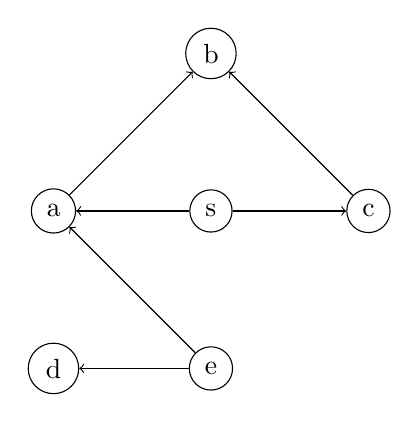
\begin{tikzpicture}[->, auto, node distance=2cm, every node/.style={circle, draw, minimum size=.5cm}]
    \node (s) {s};
    \node (a) [left of=s] {a};
    \node (b) [above of=s] {b};
    \node (c) [right of=s] {c};
    \node (d) [below of=a] {d};
    \node (e) [right of=d] {e};

    \path[every node]
    (s) edge (a)
    (s) edge (c)
    (a) edge (b)
    (c) edge (b)
    (e) edge (d)
    (e) edge (a)
    ;
  \end{tikzpicture}
  \caption{Ein gerichteter Graph}\label{fig:topo}
\end{figure}

  \begin{solution}
    Eine mögliche Topologische Sortierung ist $e, d, s, c, a, b$. Es ist möglich mehrere verschiedene Lösungen zu finden, da es sich lediglich um eine partiell Ordnung handelt.
  \end{solution}
\end{exercise}

\begin{exercise}{Kruskals Algorithmus}
  Bestimmen Sie mit Kruskals Algorithmus aus der Vorlesung einen minimalen Spannbaum für den Graphen aus \ref{fig:kruskal}. Machen Sie die Reihenfolge in der die Kanten abgearbeitet wurden deutlich.
  \begin{figure}
  \centering
  \begin{tikzpicture}[auto,on grid, node distance=2cm, vertex/.style={circle, draw, minimum size=0.75cm}]
    \node[vertex] (a) {a};
    \node[vertex, right=of a] (b) {b};
    \node[vertex, right=of b] (c) {c};
    \node[vertex, right=of c] (d) {d};
    \node[vertex, right=of d] (e) {e};
    \node[vertex, below right=2cm and 1cm of a] (f) {f};
    \node[vertex, right=of f] (g) {g};
    \node[vertex, right=of g] (h) {h};
    \node[vertex, right=of h] (i) {i};

    \draw (a) -- node {17} (b) -- node {31} (c) -- node {5} (d) -- node {23} (e) -- node {13} (i) -- node {19} (h) -- node {7} (g) -- node {23} (f) -- node {29} (a);
    \draw (b) -- node {3} (f);
    \draw (c) -- node {11} (g);
    \draw (c) -- node {13} (h);
    \draw (d) -- node {2} (h);
  \end{tikzpicture}

  \caption{Ein Beispielgraph für die Anwendung des Algorithmus von Kruskal.}\label{fig:kruskal2021}
\end{figure}

  \begin{solution}\begin{figure}
  \centering
  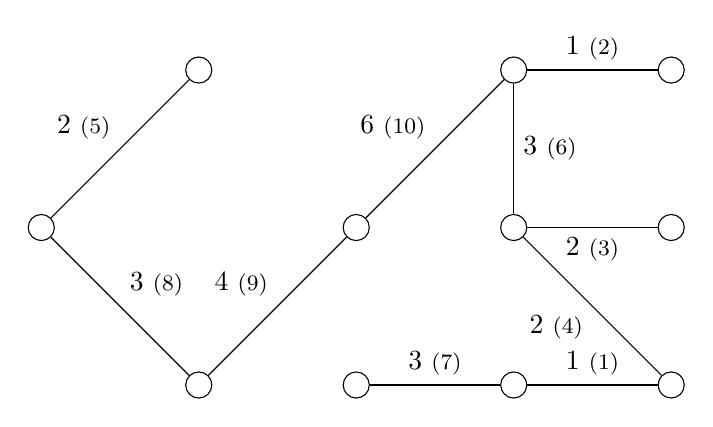
\begin{tikzpicture}[auto, node distance=2cm, main node/.style={circle, draw, minimum size=.5em}]
    \node[main node] (0) {};
    \node[main node] (1) [right of=0, below of=0] {};
    \node[main node] (2) [above of=1, above of=1] {};
    \node[main node] (3) [right of=2, below of=2] {};
    \node[main node] (4) [right of=3, above of=3] {};
    \node[main node] (5) [right of=4] {};
    \node[main node] (6) [below of=3] {};
    \node[main node] (7) [right of=6] {};
    \node[main node] (8) [right of=7] {};
    \node[main node] (9) [above of=8] {};
    \node[main node] (10) [left of=9] {};

    \path[every node]
    (7) edge node {1 \footnotesize{(1)}} (8)
    (4) edge node {1 \footnotesize{(2)}} (5)
    (9) edge node {2 \footnotesize{(3)}} (10)
    (8) edge node {2 \footnotesize{(4)}} (10)
    (0) edge node {2 \footnotesize{(5)}} (2)
    (4) edge node {3 \footnotesize{(6)}} (10)
    (6) edge node {3 \footnotesize{(7)}} (7)
    (0) edge node {3 \footnotesize{(8)}} (1)
    (1) edge node {4 \footnotesize{(9)}} (3)
    (3) edge node {6 \footnotesize{(10)}} (4)
    ;
  \end{tikzpicture}

  \caption{ein möglicher MST}\label{fig:kruskalmst}
\end{figure}\end{solution}
\end{exercise}

\begin{exercise}{Graphen}
  Betrachten Sie Graphen $G$ aus \ref{fig:simplegraph}. Wenden Sie jeweils das verlangte Verfahren an bzw. beantworten Sie die Frage oder begründen Sie, warum dies nicht geht.
  \begin{figure}
  \centering
  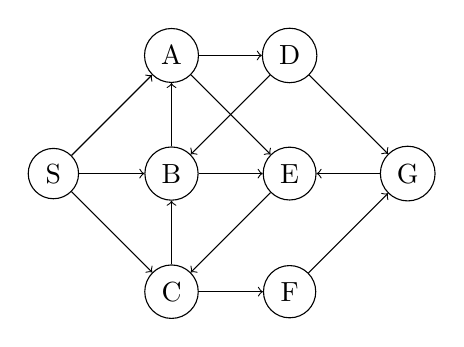
\begin{tikzpicture}[->, auto, node distance=1.5cm, every node/.style={circle, draw, minimum size=.5cm}]
    \node (S) {S};
    \node (B) [right of=S] {B};
    \node (A) [above of=B] {A};
    \node (C) [below of=B] {C};
    \node (D) [right of=A] {D};
    \node (E) [below of=D] {E};
    \node (F) [below of=E] {F};
    \node (G) [right of=E] {G};

    \path[every node]
    (S) edge (A) edge (B) edge (C)
    (A) edge (D) edge (E)
    (B) edge (A) edge (E)
    (C) edge (B) edge (F)
    (D) edge (G) edge (B)
    (E) edge (C)
    (F) edge (G)
    (G) edge (E);
  \end{tikzpicture}

  \caption{Graph $G$}\label{fig:simplegraph}
\end{figure}
  \begin{enumerate}
    \item Ermitteln Sie mit der Breitensuche einen Breitensuchbaum (BFS-Baum). Starten Sie den Algorithmus bei $s$.
    \item Ist das Ergebnis der Breitensuche eindeutig?
    \item Ermitteln Sie mit der Tiefensuche einen Tiefensuchwald und insb. die Zeiten $u.d$ und $u.f$ für jeden Knoten. Starten Sie den Algorithmus wieder bei $s$.
    \item Geben Sie eine topologische Sortierung des Graphen $G$ an.
    \item Bestimmen Sie mit dem Algorithmus aus der Vorlesung die starken Zusammenhangskomponenten von $G$. Geben Sie dazu den transponierten Graph und den Komponentengraph an.
  \end{enumerate}

  \begin{solution}
    \begin{enumerate}
      \item Ein möglicher Breitensuchbaum ist: \begin{figure}
  \centering
  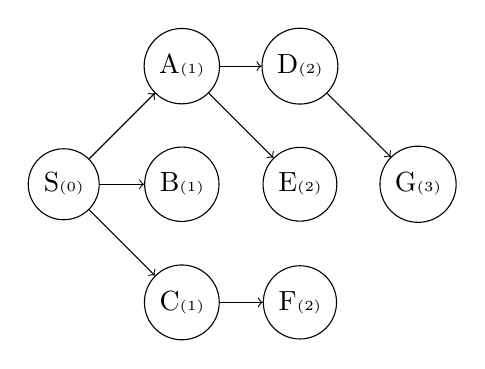
\begin{tikzpicture}[->, auto, node distance=1.5cm, every node/.style={circle, draw, minimum size=.5cm}]
    \node (S) {S\tiny{(0)}};
    \node (B) [right of=S] {B\tiny{(1)}};
    \node (A) [above of=B] {A\tiny{(1)}};
    \node (C) [below of=B] {C\tiny{(1)}};
    \node (D) [right of=A] {D\tiny{(2)}};
    \node (E) [below of=D] {E\tiny{(2)}};
    \node (F) [below of=E] {F\tiny{(2)}};
    \node (G) [right of=E] {G\tiny{(3)}};

    \path[every node]
    (S) edge (A)
    (S) edge (B)
    (S) edge (C)
    (A) edge (D)
    (A) edge (E)
    (C) edge (F)
    (D) edge (G)
    ;
  \end{tikzpicture}
\end{figure}
      \item Das Ergebnis der Breitensuche ist eindeutig.
      \item Ein möglicher Tiefensuchwald ist: \begin{figure}
  \centering
  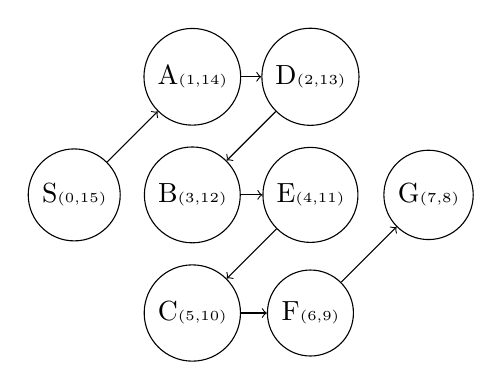
\begin{tikzpicture}[->, auto, node distance=1.5cm, every node/.style={circle, draw, minimum size=.5cm}]
    \node (S) {S\tiny{(0,15)}};
    \node (B) [right of=S] {B\tiny{(3,12)}};
    \node (A) [above of=B] {A\tiny{(1,14)}};
    \node (C) [below of=B] {C\tiny{(5,10)}};
    \node (D) [right of=A] {D\tiny{(2,13)}};
    \node (E) [below of=D] {E\tiny{(4,11)}};
    \node (F) [below of=E] {F\tiny{(6,9)}};
    \node (G) [right of=E] {G\tiny{(7,8)}};

    \path[every node]
    (S) edge (A)
    (A) edge (D)
    (D) edge (B)
    (B) edge (E)
    (E) edge (C)
    (C) edge (F)
    (F) edge (G)
    ;
  \end{tikzpicture}

  \caption{Tiefensuchwald}\label{fig:dfstree}
\end{figure}
      \item Der Graph ist kein DAG und somit gibt es keine topologische Sortierung.
      \item Die starken Zusammenhangskomponenten sind: $\{S\}, \{A, B, C, D, E, F, G\}$. \begin{table*}
  \centering
  \begin{tabular}{cc}
    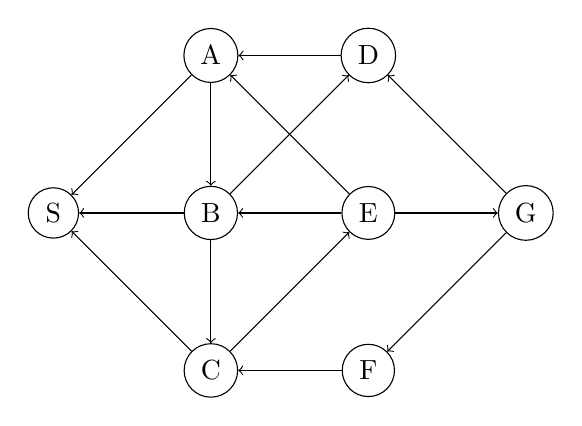
\begin{tikzpicture}[->, auto, node distance=2cm, every node/.style={circle, draw, minimum size=.5cm}]
      \node (S) {S};
      \node (B) [right of=S] {B};
      \node (A) [above of=B] {A};
      \node (C) [below of=B] {C};
      \node (D) [right of=A] {D};
      \node (E) [below of=D] {E};
      \node (F) [below of=E] {F};
      \node (G) [right of=E] {G};

      \path[every node]
      (A) edge (S) edge (B)
      (B) edge (S) edge (C) edge (D)
      (C) edge (S) edge (E)
      (D) edge (A)
      (E) edge (A) edge (B) edge (G)
      (F) edge (C)
      (G) edge (D) edge (F)
      ;
    \end{tikzpicture} &

    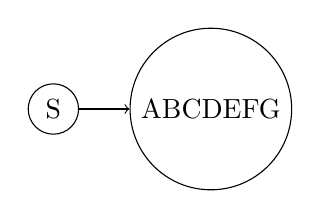
\begin{tikzpicture}[->, auto, node distance=2cm, every node/.style={circle, draw, minimum size=.5cm}]
      \node (S) {S};
      \node (ABCDEFG) [right of=S] {ABCDEFG};

      \path[every node]
      (S) edge (ABCDEFG);
    \end{tikzpicture}                     \\
    transponierter Graph                                                             & Komponentengraph
  \end{tabular}
\end{table*}
    \end{enumerate}
  \end{solution}
\end{exercise}


\begin{exercise}{Minimale Spannbäume}{\begin{figure}
  \centering
  \begin{tikzpicture}[auto, on grid, node distance=6em, main node/.style={circle, draw, minimum size=.1em}]
    \node [main node, fill=gray] (housefloorright) {};
    \node [main node] (housefloorleft) [left=of housefloorright] {};
    \node [main node] (houseroofright) [above=of housefloorright] {};
    \node [main node] (houseroofleft) [above=of housefloorleft] {};
    \node [main node] (houseroof) [above right=5em and 3em of houseroofleft] {};
    \node [main node] (treestumpleft) [right=of housefloorright] {};
    \node [main node] (treestumpright) [right=2em of treestumpleft] {};
    \node [main node] (treemidleft1) [above=2em of treestumpleft] {};
    \node [main node] (treemidright1) [above=2em of treestumpright] {};
    \node [main node] (treeleft1) [left=4em of treemidleft1] {};
    \node [main node] (treeright1) [right=4em of treemidright1] {};
    \node [main node] (treemidleft2) [above=2em of treemidleft1] {};
    \node [main node] (treemidright2) [above=2em of treemidright1] {};
    \node [main node] (treeleft2) [left=3em of treemidleft2] {};
    \node [main node] (treeright2) [right=3em of treemidright2] {};
    \node [main node] (treemidleft3) [above=3em of treemidleft2] {};
    \node [main node] (treemidright3) [above=3em of treemidright2] {};
    \node [main node] (treeleft3) [left=2em of treemidleft3] {};
    \node [main node] (treeright3) [right=2em of treemidright3] {};
    \node [main node] (treetop) [above right=4em and 1em of treemidleft3] {};

    \path[every node]
    (housefloorright) edge node {5} (housefloorleft) edge node [below right=.5 and .1] {5} (houseroofleft) edge node {3} (houseroofright) edge node [below] {1} (treestumpleft)
    (housefloorleft) edge node {3} (houseroofleft) edge node [above right=.5 and .1] {4} (houseroofright)
    (houseroofright) edge node [above] {20} (houseroofleft) edge node [above right] {-3} (houseroof)
    (houseroofleft) edge node {6} (houseroof)
    (treestumpleft) edge node [below] {2} (treestumpright) edge node {4} (treemidleft1)
    (treestumpright) edge node [right] {1} (treemidright1)
    (treemidleft1) edge node {9} (treemidright1) edge node {5} (treeleft1)
    (treemidright1) edge node [below] {3} (treeright1)
    (treeleft1) edge node [left] {6} (treemidleft2)
    (treeright1) edge node [right] {4} (treemidright2)
    (treemidleft2) edge node [above] {7} (treeleft2)
    (treemidright2) edge node {5} (treeright2)
    (treeleft2) edge node [left] {1} (treemidleft3)
    (treeright2) edge node [right] {-2} (treemidright3)
    (treemidleft3) edge node [above] {2} (treeleft3)
    (treemidright3) edge node {1} (treeright3)
    (treeleft3) edge node {6} (treetop)
    (treeright3) edge node [above right] {8} (treetop)
    ;
  \end{tikzpicture}

  \caption{Graph $G$}\label{fig:mstgraph}
\end{figure}}
  \begin{enumerate}
    \item Bestimmen Sie mit Hilfe des Algorithmus von Prim einen minimalen Spannbaum des Graphen aus \ref{fig:mstgraph} und skizzieren diesen. Der Startknoten ist grau gefärbt. Geben Sie zusätzlich die Reihenfolge an, in der die Kanten des Spannbaums gemäß Algorithmus hinzugefügt werden.
    \item Sei $G = (V, E)$ ein zusammenhängender gewichteter Graph mit Gewichtsfunktion $w : E \rightarrow \mathbb{R}$ und $T = (V, E_0)$ ein minimaler Spannbaum von $G$.
          \begin{enumerate}
            \item Für eine beliebige Kante $e \in E \setminus E_0$ wird deren Gewicht $w(e)$ erhöht. Wir bezeichnen diesen modifizierten Graphen als $G'$. Zeigen Sie, dass $T$ ebenfalls ein minimaler Spannbaum von $G'$ ist.
            \item Für eine beliebige Kante $e \in E$ wird deren Gewicht $w(e)$ verringert. Wir bezeichnen diesen modifizierten Graphen als $G'$. Konstruieren Sie einen Algorithmus, welcher einen minimalen Spannbaum von $G'$ mit Hilfe von $T$ in Zeit $\bigO(|V| + |E|)$ berechnet.
                  \hint{Hier ist kein Pseudocode gefordert.}
          \end{enumerate}
  \end{enumerate}

  \begin{solution}
    \begin{enumerate}
      \item Ein möglicher minimaler Spannbaum ist: \begin{figure}
  \centering
  \begin{tikzpicture}[auto, on grid, node distance=6em, main node/.style={circle, draw, minimum size=.1em}]
    \node [main node, fill=gray] (housefloorright) {};
    \node [main node] (housefloorleft) [left=of housefloorright] {};
    \node [main node] (houseroofright) [above=of housefloorright] {};
    \node [main node] (houseroofleft) [above=of housefloorleft] {};
    \node [main node] (houseroof) [above right=5em and 3em of houseroofleft] {};
    \node [main node] (treestumpleft) [right=of housefloorright] {};
    \node [main node] (treestumpright) [right=2em of treestumpleft] {};
    \node [main node] (treemidleft1) [above=2em of treestumpleft] {};
    \node [main node] (treemidright1) [above=2em of treestumpright] {};
    \node [main node] (treeleft1) [left=4em of treemidleft1] {};
    \node [main node] (treeright1) [right=4em of treemidright1] {};
    \node [main node] (treemidleft2) [above=2em of treemidleft1] {};
    \node [main node] (treemidright2) [above=2em of treemidright1] {};
    \node [main node] (treeleft2) [left=3em of treemidleft2] {};
    \node [main node] (treeright2) [right=3em of treemidright2] {};
    \node [main node] (treemidleft3) [above=3em of treemidleft2] {};
    \node [main node] (treemidright3) [above=3em of treemidright2] {};
    \node [main node] (treeleft3) [left=2em of treemidleft3] {};
    \node [main node] (treeright3) [right=2em of treemidright3] {};
    \node [main node] (treetop) [above right=4em and 1em of treemidleft3] {};

    \path[every node]
    (housefloorright) edge node {3\tiny{(4)}} (houseroofright) edge node [below] {1\tiny{(1)}} (treestumpleft)
    (houseroofright) edge node [above left] {4\tiny{(7)}} (housefloorleft) edge node {-3\tiny{(5)}} (houseroof)
    (housefloorleft) edge node {3\tiny{(8)}} (houseroofleft)
    (treestumpleft) edge node [below] {2\tiny{(2)}} (treestumpright) edge node {4\tiny{(9)}} (treemidleft1)
    (treestumpright) edge node [right] {1\tiny{(3)}} (treemidright1)
    (treemidright1) edge node [below right] {3\tiny{(6)}} (treeright1)
    (treemidleft1) edge node [below left] {5\tiny{(11)}} (treeleft1)
    (treeright1) edge node [left] {4\tiny{(10)}} (treemidright2)
    (treeleft1) edge node [right] {6\tiny{(15)}} (treemidleft2)
    (treemidright2) edge node [below right] {5\tiny{(12)}} (treeright2)
    (treemidleft2) edge node [below left] {7\tiny{(16)}} (treeleft2)
    (treeright2) edge node [left] {-2\tiny{(13)}} (treemidright3)
    (treeleft2) edge node [right] {1\tiny{(17)}} (treemidleft3)
    (treemidright3) edge node [below right] {1\tiny{(14)}} (treeright3)
    (treemidleft3) edge node [below left] {2\tiny{(18)}} (treeleft3)
    (treeleft3) edge node [left] {6\tiny{(19)}} (treetop)
    ;
  \end{tikzpicture}

  \caption{Ein MST des Graphen.}
\end{figure}
      \item \begin{enumerate}
              \item Sei $T = (V, E_0)$ ein minimaler Spannbaum von $G = (V, E)$ und $G' = (V, E')$ ein modifizierter Graph. Sei $T' = (V, E_0')$ ein minimaler Spannbaum von $G'$. Es gilt $E_0 \subseteq E'$. Da $T$ ein minimaler Spannbaum von $G$ ist, gilt $w(E_0) \leq w(E')$. Da $T'$ ein minimaler Spannbaum von $G'$ ist, gilt $w(E_0') \leq w(E')$. Da $E_0 \subseteq E_0'$, gilt $w(E_0) \leq w(E_0')$. Insgesamt folgt $w(E_0) \leq w(E_0') \leq w(E')$, also ist $T$ auch ein minimaler Spannbaum von $G'$.
              \item Der Algorithmus arbeitet wie folgt: \begin{itemize}
                      \item[$\bigO(E)$] Finde die veränderte Kante.
                      \item Falls in $T$ enthalten, passe das Gewicht an.
                      \item[$\bigO(V+E)$] Sonst suche den Pfad (zB. BFS) von $e.u$ zu $e.v$ in $T$. Wenn $w(e) < w(f)$ für eine Kante $f$ auf dem Pfad, ersetze $f$ durch $e$.
                    \end{itemize}
                    Dadurch wird ein minimaler Spannbaum von $G'$ in Zeit $\bigO(V+2E)=\bigO(V+E)$ berechnet.
            \end{enumerate}
    \end{enumerate}
  \end{solution}

\end{exercise}

\begin{exercise}{Brückenkanten}
  Eine Kante $e \in E$ eines zusammenhängenden, ungerichteten Graphen $G = (V, E)$ heißt Brückenkante, falls der Graph $G_0 = (V, E \setminus \{e\})$, der durch das Entfernen der Kante $e$ aus $G$ entsteht, nicht mehr zusammenhängend ist.
  \begin{figure}
  \centering
  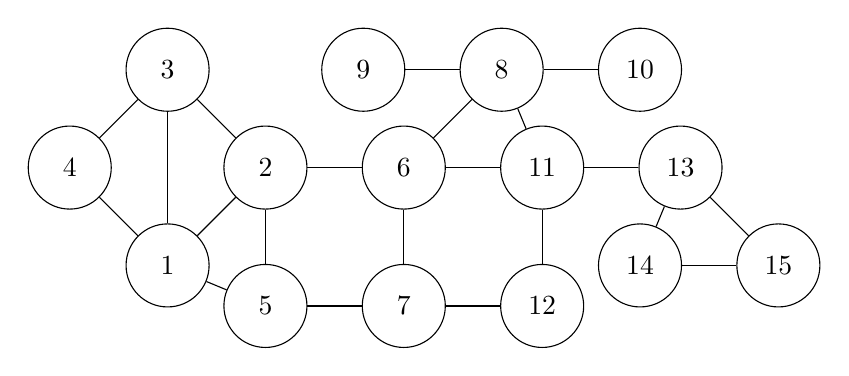
\begin{tikzpicture}[auto, node distance=5em, main node/.style={circle, draw, minimum size=3em}]
    \node (1) [main node] {1};
    \node (2) [main node, above right of=1] {2};
    \node (3) [main node, above left of=2] {3};
    \node (4) [main node, above left of=1] {4};
    \node (5) [main node, below of=2] {5};
    \node (6) [main node, right of=2] {6};
    \node (7) [main node, right of=5] {7};
    \node (8) [main node, above right of=6] {8};
    \node (9) [main node, left of=8] {9};
    \node (10) [main node, right of=8] {10};
    \node (11) [main node, right of=6] {11};
    \node (12) [main node, right of=7] {12};
    \node (13) [main node, right of=11] {13};
    \node (14) [main node, below right of=11] {14};
    \node (15) [main node, right of=14] {15};

    \path[every node]
    (1) edge (2) edge (3) edge (4) edge (5)
    (2) edge (3) edge (5) edge (6)
    (3) edge (4)
    (5) edge (7)
    (6) edge (7) edge (8) edge (11)
    (7) edge (12)
    (8) edge (9) edge (10) edge (11)
    (11) edge (12) edge (13)
    (13) edge (14) edge (15)
    (14) edge (15)
    ;
  \end{tikzpicture}

  \caption{Graph $G$}\label{fig:bridgegraph}
\end{figure}
  \begin{enumerate}
    \item Bestimmen Sie alle Brückenkanten im abgebildeten Graphen aus \ref{fig:bridgegraph}.
    \item Geben Sie einen Algorithmus in Pseudocode an, der in Laufzeit $\bigO(|V| \cdot |E| + |E|^2)$ entscheidet, ob ein zusammenhängender, ungerichteter Graph $G$ eine Brückenkante besitzt oder nicht.
    \item Zeigen Sie, dass Ihr Algorithmus korrekt arbeitet.
    \item Zeigen Sie, dass Ihr Algorithmus die Laufzeitschranke einhält.
  \end{enumerate}

  \begin{solution}
    \begin{enumerate}
      \item Die Brückenkanten sind: $(11-13) (8-9) (8-10)$.
      \item Der Algorithmus findBridges kann genutzt werden indem $false$ zurückgegeben wird, wenn die Menge der Brückenkanten $B$ leer ist. Andernfalls wird $true$ zurückgegeben.\par
            \begin{alg}
  \signed{findBridges}{G}{B}
  \params{A graph $G$}{A list of bridges $B$}

  $B \gets \emptyset$\;
  $s \gets G.V.first$\;
  \ForEach{edge $e\in G.E$}{
    $ICC \gets$ \texttt{findICC($G\setminus \{e\}, s$)}\explain*{an initial connected component describes the vertices reachable from $s$}
    \lIf{$|ICC.V| < |G.V|$}{$B \gets B \cup \{e\}$}
  }
  \Return $B$\;
\end{alg}

      \item Der Algorithmus arbeitet korrekt, da er für jede Kante $e$ prüft, ob der Graph $G_0$ nach Entfernen von $e$ noch zusammenhängend ist.
      \item Die Laufzeit des Algorithmus ist $\bigO(|V| \cdot |E| + |E|^2)$, da die DFS in $\bigO(|V| + |E|)$ arbeitet und die diese für jede Kante $e$ in $\bigO(|E|)$ aufgerufen wird.
    \end{enumerate}
  \end{solution}
\end{exercise}

\begin{exercise}{Dijkstras Algorithmus}{\begin{figure}
  \centering

  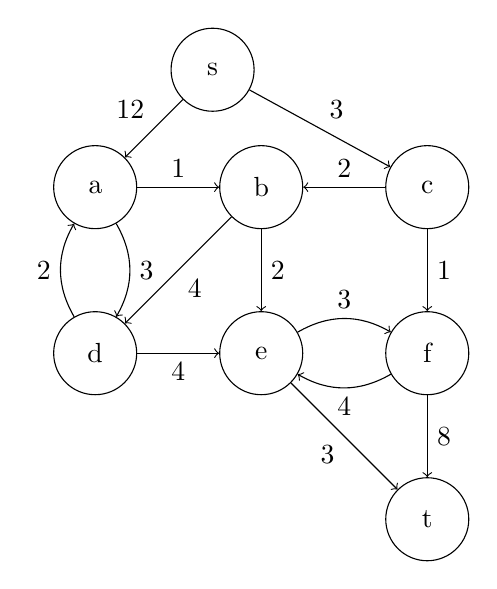
\begin{tikzpicture}[->, auto, node distance=6em, main node/.style={circle, draw, minimum size=3em}]
    \node (s) [main node] {s};
    \node (a) [main node, below left of=s] {a};
    \node (b) [main node, right of=a] {b};
    \node (c) [main node, right of=b] {c};
    \node (d) [main node, below of=a] {d};
    \node (e) [main node, right of=d] {e};
    \node (f) [main node, right of=e] {f};
    \node (t) [main node, below of=f] {t};

    \path[every node]
    (s) edge node [above left] {12} (a)
    (s) edge node {3} (c)
    (a) edge node {1} (b)
    (c) edge node [above] {2} (b)
    (a) edge [bend left] node {3} (d)
    (d) edge [bend left] node {2} (a)
    (b) edge node {4} (d)
    (d) edge node [below] {4} (e)
    (b) edge node {2} (e)
    (c) edge node {1} (f)
    (e) edge [bend left] node {3} (f)
    (f) edge [bend left] node {4} (e)
    (e) edge node [below left] {3} (t)
    (f) edge node {8} (t)
    ;
  \end{tikzpicture}

  \caption{Graph $G$}\label{fig:dijkstra}
\end{figure}}
  \begin{enumerate}
    \item Wenden Sie Dijkstras Algorithmus auf den Graphen aus \ref{fig:dijkstra} an. Beginnen Sie bei Knoten $s$. Geben Sie tabellarisch die am Ende jeder Iteration der While-Schleife in der Queue enthaltenen Keys an.
    \item Modifizieren Sie den Pseudocode von Dijkstras Algorithmus so, dass er als Input einen Graphen, einen Startknoten $s$ und einen Zielknoten $v$ als Input nimmt und als Output die explizite Darstellung des kürzesten Pfades von $s$ nach $v$ als Sequenz von Knoten ausgibt. Begründen Sie kurz die Korrektheit Ihrer Lösung. Die Laufzeit des modifizierten Algorithmus darf dabei nicht die asymptotische Laufzeitschranke $\bigO(V \log V + E)$ des Dijkstra Algorithmus überschreiten.
  \end{enumerate}

  \begin{solution}
    \begin{enumerate}
      \item Die Queue enthält am Ende jeder Iteration die Keys: \begin{table}
  \begin{tabular}{c|l}
    $i$ & Queue                                                                    \\
    \hline
    0   & $\{s^0,a^\infty,b^\infty,c^\infty,d^\infty,e^\infty,f^\infty,t^\infty\}$ \\
    1   & $\{c^3,a^{12},b^\infty,d^\infty,e^\infty,f^\infty,t^\infty\}$            \\
    2   & $\{f^4,b^5,a^{12},d^\infty,e^\infty,t^\infty\}$                          \\
    3   & $\{b^5,e^8,a^{12},t^{12},d^\infty\}$                                     \\
    4   & $\{e^7,d^9,a^{12},t^{12}\}$                                              \\
    5   & $\{d^9,t^{10},a^{12}\}$                                                  \\
    6   & $\{t^{10},a^{11}\}$                                                      \\
    7   & $\{a^{11}\}$                                                             \\
    8   & $\{\}$                                                                   \\
  \end{tabular}

  \caption{Queue nach jeder Iteration in Dijkstras Algorithmus}\label{tbl:dijkstra}
\end{table}
      \item Der modifizierte Algorithmus arbeitet wie folgt: \begin{itemize}
              \item Führe Dijkstras Algorithmus aus.
              \item Wenn $v$ erreicht wurde, konstruiere den Pfad von $s$ nach $v$ durch Rückverfolgung der Vorgänger.
            \end{itemize}
            Die Laufzeit des modifizierten Algorithmus ist $\bigO(V \log V + E)$, da die Rückverfolgung der Vorgänger in $\bigO(V)$ arbeitet.
    \end{enumerate}
  \end{solution}
\end{exercise}

\end{document}